\chapter{Designing and Implementing \AspectOriented{} Models}
\label{chap:exp1_simulation_optimisation}
\label{chap:experiment_setup}


This chapter describes the design and implementation of experiments which
investigate using advice to augment behaviour in a model. The experiments
simulate RPGLite gameplay. Using these simulations, the experiments investigate
the utility of \aop{} in a simulation \& modelling context. Advice which uses
data about players' gameplay~\cite{rpglite_dataset} is applied to a basic model
of RPGLite play. The advice changes the behaviour of simulated players in an
attempt to reflect realistic interactions with the game. The behaviour modified
by the advice is players' selection of character pairs. Character pairs selected
by simulated players are compared against those from a player's gameplay data
and their correlation is measured. If the datasets correlate, then players are
successfully simulated. This approach is used to answer the research
questions proposed in \cref{chap:lit_review}: 

\Needspace{6\baselineskip}
\begin{researchquestion}
  \begin{description}
   \item[RQ1] \rqtwo{}
   \item[RQ2] \rqthree{}
   \item[RQ3] \rqfour{}
  \end{description}
\end{researchquestion}

To answer these, two approaches to modifying player behaviour are developed:
one alters the distribution from which character pairs are selected to reflect
the distribution found in a player's gameplay data, 
and the other models the player learning to play RPGLite and developing
preferences for certain character pairs in the process.

The experiments share a significant proportion of their design and
implementation. As their common elements require a significant amount of
explanation, a chapter outlining both the setup \emph{and} results of these
experiments would be extremely long, and their shared foundation means that they
are most naturally explained together. For this reason, the design and
implementation of \emph{all} experiments is explained in this chapter, and their
results follow in \cref{chap:experimental_results}.

The common aspects of design and implementation in this chapter are explored as
follows. To give context as to how different pieces of the experiments'
foundations are used, an overview of the models constructed and the experiments
employing them is given in \cref{experiment_design_sec_models_and_experiments}.
The model of RPGLite play which these experiments weave aspects into is
described in \cref{sec:naive_model}. The design of the more complex of the two
models of behaviour change --- a model of learning --- is explained in
\cref{learning_model_definition}. Aspects implementing the learning model, other
models of behavioural change, and additional apparatus required to conduct
experiments are described in \cref{aspects_applied_section}. Having described
details of the aspects used by experiments, details of the implementation of the
experiments themselves are given in
\cref{sec:optimisation_with_aspects_experimental_design}. Following this,
\cref{chap:experimental_results} explains the design, implementation, results
and evaluation of each experiment individually, as all context necessary to
understand these designs and evaluations are given in the aforementioned
sections.

\section{Experiment Design}
\label{experiment_design_sec_models_and_experiments}

To answer the proposed research questions, two models are made which change
simulated players' character pair selections: one which reflects the choices
made by the player being simulated, and another which simulates that player
learning over time. These are used to examine three things about
\aspectoriented{} simulations \& models: whether aspects can be woven to improve
a model's accuracy; whether it is feasible to use aspects to introduce new
behaviours and parameters in a model; and whether the same aspects can be
successfully woven across different models.


The complete designs for the first, second, and third experiments are explained
in \cref{sec:rq2}, \cref{sec:rq3}, and \cref{sec:rq4} respectively as it is
useful to have discussed the implementation of the RPGLite model, aspects, and
statistical methodologies before the experimental design is explained. However,
some context as to how those foundations are used is important when explaining
them too. For this reason, a brief description of the behavioural modifications
and the experiments which use them are given here, and more detailed
descriptions are given in the following chapter.

\subsection{Changes to Behaviour}

Simulated players' behaviour is changed using aspects when they select
characters. The rationale for altering character selection in particular is
explained in \cref{learning_model_definition}. The model they alter ---
described in \cref{sec:naive_model} --- is ``naive'', meaning that it makes all
decisions a player could make randomly rather than strategically or optimally.
Two changes to character pair selection are created: the first selects
characters with the same distribution as found the gameplay data of a player
being simulated, called the ``prior distribution'' model; the second selects
characters by modelling players learning which characters are most likely to win
games and selecting character pairs according to what they learned, called the
``learning model''.

\Needspace{3\baselineskip}
\begin{description}
\item[Prior Distribution Model] The prior distribution model selects character
pairs with a distribution calculated from players' gameplay data.\footnote{The
distribution is known ahead of the simulation being run, hence ``prior''.} As
the distribution is already known, simulated games can reproduce the
distribution. This makes little change to the behaviour of simulated players, as
no new activity is modelled on their part: no additional actions are taken and
simulated players do not behave in a ``new'' way. However, the emergent
properties of simulated play should reflect the dataset used by the prior
distribution model. This is expected to have the effect of synthesising new
datasets with the same emergent properties and requires little modification to
the model. The implementation of the prior distribution model is given in
\cref{prior_distribution_aspect_description}.

\item[Learning Model] The learning model selects character pairs by preferring
pairs which previously won games. This model requires an additional model of
confidence to support it (discussed in \cref{subsec:confidence_model}) and
special measures to be in place when generating datasets to ensure the space of
possible character pairs is explored properly (discussed in
\cref{subsec:controlling_state_space_exploration}). As a result this explanation
is superficial and is provided as necessary context for the introduction of
experiments following in \cref{experiments_introduced_briefly}. A thorough
discussion of the learning model is given in \cref{learning_model_definition}.

The learning model selects character pairs using a distribution defined by the
pairs' number of observed wins. If a player has never seen a character pair
winning a game, that pair is unlikely to be selected; if a player sees a pair
winning an overwhelming number of games, the pair will be selected
proportionally to its win rate. This model introduces new behaviours for
simulated players, as their decisions are based on historical observations which
are not present in the original model and emerge from a player's interactions
with others as opposed to being defined when the model is first executed.
New parameters are also introduced to control how players learn, including a
parameter controlling their arrogance, a parameter scaling the number of games
required for them to rely on their knowledge, and parameters controlling how
bored they are and how likely they are to stop playing RPGLite. The introduction
of new behaviours and parameters to the naive model allows the latter two
research questions to be answered.

 
\end{description}



\subsection{Brief Explanations of Experiments}
\label{experiments_introduced_briefly}

\Needspace{3\baselineskip}
\begin{description}
  \item[Experiment \#1: Improving a Model] The first experiment answers the
research question: \emph{\rqtwo{}} \Aop{} can only be used to augment models if
modifications to a model can be encoded in aspects, woven into a model, and
become provably more accurate as a result. Similar research was conducted in
prior work~\cite{wallis2018caise}, but this study represented changes to a model
which were not verified as ``accurate'' or ``realistic''. Beyond producing a
change that \emph{looked} accurate, it did not simulate any real-world system
and so could not be verified as rigorously as a model of RPGLite gameplay can
be.

To verify that a model is changed in the intended way through the weaving of
advice, three datasets of completed games are used for each player simulated.
The first is that player's gameplay data collected from their interactions with
the mobile game in RPGLite's first season, the second is produced by the naive
model, and the third is produced by the naive model with the prior distribution
model woven. The distribution of character pairs chosen by each model is
compared with the player's distribution of character pairs chosen using a
correlation metric explained in \cref{measuring_charpair_similarity}. The random
distribution of chosen pairs produced by the naive model is expected to
correlate poorly with the player's distribution of choices, as the player is
expected to be biased toward certain character pairs as they continue to play
RPGLite. The prior distribution model should produce datasets with the same
distribution as the player exhibited when interacting with the mobile game, so
the dataset produced with the prior distribution model woven into RPGLite should
correlate closely to the empirically sourced dataset. If this behaviour is seen,
then the aspects woven into the model induced a change in simulated players'
behaviours and so successfully augmented the model \laurie{devil's advocate:
this may not be `successful' or `augment': it could be an unsuccessful change (in the sense of ``change that we didn't want'')}.

A more thorough description of this experiment is given in \cref{sec:rq2} as the
reader has been presented with the details of the experiment's foundation at
that point.
  
  \item[Experiment \#2: Extending Behaviours in a Model] The first experiment
investigates whether advice can alter a model and introduce changes to existing
behaviours. Another experiment follows to investigate whether advice can
introduce \emph{new} behaviours to a model and new parameters which alter
modelled behaviour. This aims to answer the research question:
\emph{\rqthree{}}

The learning model is woven into the naive model of RPGLite play to add new
behaviours and parameters to the model. For each player, parameters are found
using a technique explained in
\cref{identifying-significant-results-explanation} which simulate their learning
most accurately. This technique determines reproducible results which show
statistically significant correlation with the player's gameplay data from the
RPGLite mobile game, extending the statistics used in the first experiment
(explained in \cref{measuring_charpair_similarity}). If the learning model can
reproduce the play style of some real-world players, then the additional
behaviour and parameters successfully model their play of RPGLite and the
experiment is a success. To do this, datasets are generated by weaving the
learning model parameterised in different ways. The correlation of these
datasets is measured against subsets of a player's season 1 gameplay data. If
the parameters can produce data which correlates with the player's gameplay data
consistently, the player is accurately simulated by the learning model with
these parameters and so the research question is answered.

Note that not all players are expected to be simulated accurately by the model
of learning. For example, players might have biases toward or against some
characters, might play in cliques which limit their exploration of possible
character pairs, or might learn differently to the way the model assumes such as
exhibiting temporal
discounting~\cite{green1996exponential_versus_hyperbolic_discounting}. As these
experiments aim to investigate the feasibility of applying \aop{} in a
simulation \& modelling context, building a formalism of learning which is
universally applicable to all players is beyond the project's scope. The
experiment only seeks to demonstrate that new behaviours \emph{can} be
accurately represented by advice, and that the technique can be used in future
work to augment models in whatever manner a research team requires.

A more thorough description of this experiment is given in \cref{sec:rq3}, as the
reader has been presented with the details of the experiment's foundation at
that point.



\item[Experiment \#3: Behaviours as Cross-Cutting Concerns] Having conducted the
first two experiments, the utility of aspects as units of behaviour change are
established. The results in \cref{sec:rq2} and \cref{sec:rq3} are positive. One
more research question remains to be addressed. The final research question is:
\emph{\rqfour{}}

To establish this, season 2 of RPGLite is used to represent a system
which is subtly changed. RPGLite's seasons are defined by game configurations,
which means that the behaviours of players do not change but the strengths and
weaknesses of different characters do. To play strategically, players must learn
which changes have affected their ordinary strategies and re-evaluate their
preferred character pairs. The prior distribution model and learning model
should work independently of the RPGLite season they are applied to, and so ---
given positive results are found for the first and second experiments --- the
models ought to work when woven into a model of the second season
too.

Data is generated using the prior distribution model and learning model in the
same manner as in earlier experiments, but applied to player's gameplay data
from RPGLite's second season. Parameters which yielded statistically significant
results for the learning model in season 1 are used in season 2, as these
parameters ought to represent how an individual player learns. The learning
model may also work to simulate season 2 players, but with different parameters;
to investigate this, model parameters specific to season 2 are found which yield
statistically significant datasets using the same technique as in the second
experiment. If these aspectually-augmented models successfully simulate players
then the experiment establishes the portability of aspects representing
behavioural change. Correlation is measured in the same ways as in previous
experiments to evaluate the models' accuracy in simulating players.

A more thorough description of this experiment is given in \cref{sec:rq4} as the
reader has been presented with the details of the experiment's foundation at
that point.


\end{description}



\section{Naive Model}\label{sec:optimisation_with_aspects_naivemodel}
\label{sec:naive_model}

A naive model of play was developed by separating each stage of the actions
taken by players and separating them into individual procedures. The model was
written as a workflow in Python, and state of workflow execution was separated
into three components: the actor that a function invocation (or ``step'')
represents activity from; a ``context'' in the parlance of languages like
Golang, representing the state of a game being played; and the environment in
which that game is played.\footnote{Incidentally, this structure allowed a
flexible and natural implementation of a procedural simulation containing
concepts common in software engineering (such as contexts) and environments
(found in simulation frameworks). We imagine that it is easily adopted in
existing simulation frameworks such as SimPy\cite{simpy_intro}. Some additional
detail is included in \cref{appendix_ace_pattern}.} The naive model of RPGLite
follows a simple workflow mimicking player interaction with the mobile game
deployed. A graphical representation is provided in \cref{fig:naive_model}.
\Cref{fig:naive_model_with_experimental_apparatus} contains a diagram showing
how the naive model is used to produce synthetic data by simulating repeated
gameplay.

\begin{figure}[tp]
  \centering
  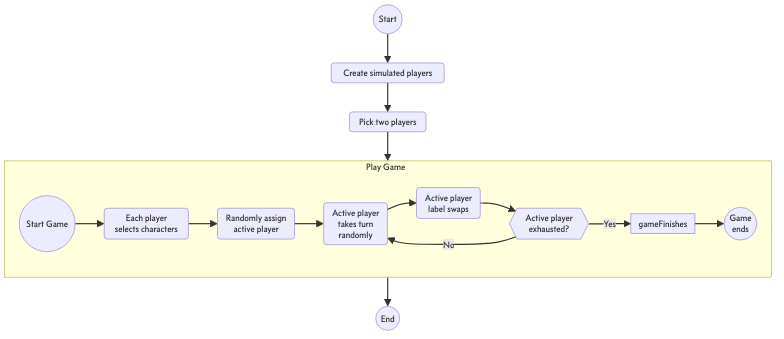
\includegraphics[width=\columnwidth]{60_optimisation_with_aspects/diagrams/naive_model.png}
  \caption{A diagram of the ``naive model'' of RPGLite play used in experiments.}
  \label{fig:naive_model}

  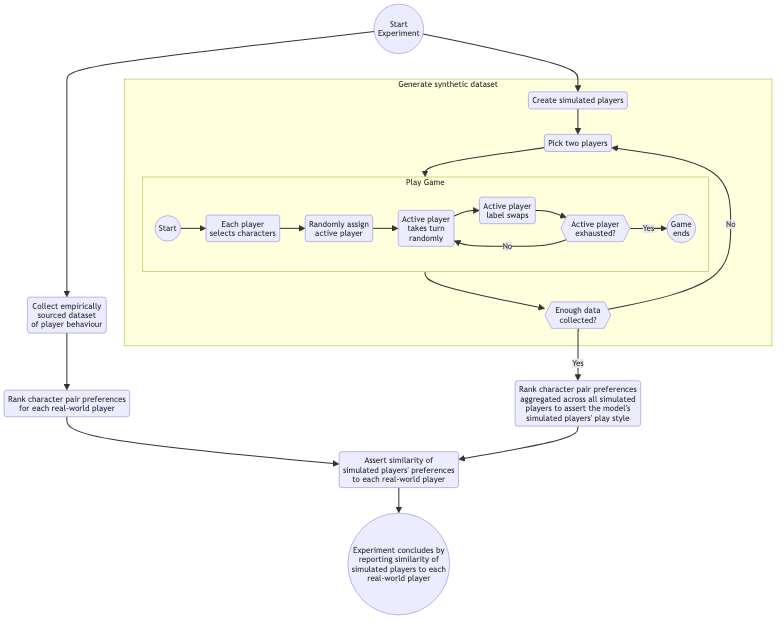
\includegraphics[width=\columnwidth]{60_optimisation_with_aspects/diagrams/experiment_setup_for_datagen.png}
  \caption{A diagram illustrating how the naive model is used to generate datasets used in experiments.}
  \label{fig:naive_model_with_experimental_apparatus}
\end{figure}


\inline{Move mermaid-based figures to .svg for fidelity}

Two randomly-selected players repeatedly select characters to play from the pool
of 8 characters described in \cref{chap:rpglite}, and a player is chosen to play
first at random, referred to as the ``active'' player. That player selects a
random valid move to make. The active player alternates, and the process
repeats, until such time as an active player starts their turn with both of
their characters fully depleted of health. The player with remaining characters
is the victor. When used to generate datasets for analysis, another game is
started by picking another pair of random players and starting a game between
them; this continues until a predetermined number of games has been played.
After a sufficient number of games are played, analysis of the generated datasets
is performed. \footnote{Dataset analysis is explained in
\cref{sec:optimisation_with_aspects_experimental_design}.}
Decisions made by players in the model are random; this is because the model is
designed to avoid informed decisions where possible. This model illustrates the
steps taken by players and disregards whether the simulated players' choices
reflect realistic ones. Informed decisions are woven as \aspectoriented{}
changes to behaviour.

\inline{
  There's more I can and should write here. For example, how are seasons
  represented? How do we switch between them? I also have classes representing
  individual characters etc\ldots{}
}





\section{Modelling Learning}
\label{learning_model_definition}

The naive model makes choices randomly. Informed decisions are made by weaving
advice into the model which changes player behaviour. Experiments are evaluated
through the distribution of character pairs found in gameplay data, so aspects
are required which change that distribution of character pairs. To change the
distribution of character pairs chosen, an \aspectoriented{} model of learning
is created which alters player behaviour to select character pairs at the
beginning of a game by inferring strong characters from those observed to win
games previously. This section describes its design.

\subsection{What Players Learn}

Players learn many things when playing a game. Other than learning about
characters and their strengths and weaknesses, players also learn how to take
successful turns by making moves strategically. Character pair selection is the
focus of these experiments because they are simpler and have a smaller state
space for players to understand: the ``metagame'' for character pair selections
is the simpler of the two.

\label{metagame_explanation}
A metagame is a community's perception of ``good'' gameplay at a given point in
time. For example, if certain characters are popular, players may select other
characters which are not likely to win against \emph{most} characters but are
likely to win against \emph{currently popular} ones. As a result, players may
select weak characters strategically, and strategically selected characters
change over time in response to changing popular choices in the community.
Similar reasoning applies to move selection. For a more thorough discussion of
the concept of a metagame, see the survey of literature and definitions by
\citet{metagaming_in_esports} or the original but more theoretical work on the
topic by \citet{howard1971metagames_seminal}.

\label{modelling_char_selection_instead_of_move_selection}
A design consideration of RPGLite is that its metagame is ``solvable'', meaning
that there exists an objectively optimal choice for a player to make in any
state~\cite{kavanagh2021thesis}. As the space of possible moves is much larger
than the space of possible character pair choices players are expected to learn
optimal choices more quickly, which would lead to an unchanging (``stable'')
metagame. In practice, the character selection metagame converged on optimal
character selections, whereas players consistently made errors when selecting
optimal moves~\cite{kavanagh2021gameplay}. As players' choices of character
pairs is therefore easier to model (and more consistent between players), a
model of learning is applied to their character pair selections instead of their
move selections. Player behaviour is altered to select objectively optimal moves
in every state instead of this being learned over time; this is described in
\cref{aspect_to_ensure_best_move}.



\subsection{Literature regarding Learning}
\label{subsec:models_of_learning_discussed}

Different people learn in different ways. Indeed, no universally-accepted
definition of learning appears to exist. This is presumably because it is
convenient to define what it means to learn differently in the context of
different pieces of work. For example, cognitive models of learning can be
useful when considering mental processes specifically, whereas functional models
of learning lend a more empirically applicable perspective. What it means to
learn is outwith the scope of this research; however, the experiments presented
in \cref{chap:experimental_results} include a model of learning. To justify our
model, we consider a functional approach to learning, as this is more closely
linked to the empirically focused work of simulating real-world behaviour than
cognitive alternatives.

\citet{lachman1997learning} summarises standard definitions of learning as
``\textelp{} a relatively permanent change in behavior as a result of practice
or experience''. They observe that these definitions have practical shortcomings
such as a focus on behavioural change (as learning may not change behaviour) or
conflating learning's process and its product (the process by which we learn is
not obviously identical to its result, of which behavioural change is an
example). They suggest learning might be better defined as:

\begin{displayquote}
\textelp{} the process by which a relatively stable modification in
stimulus-response relations is developed as a consequence of functional
environmental interaction via the senses [\ldots{}] rather than as a consequence
of mere biological growth and development~\cite{lachman1997learning}.
\end{displayquote}

They note that their definition distinguishes learning from phenomena such as
injury, changes to one's maturity, or sensory adaptation, incorporates
stimulus-response relationships the research community consider as learned, and
differentiates learning's process and product. Their model is inherently
functional, making it useful for the purposes of simulation and modelling,
although they offer only a definition of learning and a brief comparison to
the standard textbook definition they introduce. The work presented is not
intended to demonstrate its improved model of learning empirically, only to
discuss its semantic merit. However, the models proposed in this thesis require
only a theoretically informed, sound basis for their model of learning, and a
lack of empirical justification is not a barrier to the relevance of the model
\citeauthor{lachman1997learning} proposes.

\citet{de2013learning} propose a functional definition of learning which is
primarily concerned with providing a definition of learning which is both
accurate and useful for the purposes of cognitive learning research. Doing so
attempts to provide a model around which some consensus can be reached; learning
is a central concept in psychology, and they describe their definition as
supportive of cognitive work without requiring a cognitive model. They introduce
their definition as:

\begin{displayquote}
Our definition consists of three components: (1) changes in the behavior of the
organism, (2) a regularity in the environment of the organism, and (3) a causal
relation between the regularity in the environment and the changes in behavior
of the organism.
\end{displayquote}

This model of learning contains more nuance than the ``textbook definitions'' of
learning they paraphrase as ``a change in behaviour that is due to experience''
but does not stray far from the core concept of an environmental stimulus
impacting behaviour in a causal fashion. The introduction of ``regularity'' to
their definition refers to the presence of the stimulus with some form of
repetition, either through multiple instances of a stimulus at different times
or the same stimulus occurring concurrently. \citet{de2013learning} observe that
their model is straightforward without the sweeping inclusivity of the simple
model mentioned earlier and is easily verified (although, as in the work of
\citet{lachman1997learning}, empirical verification is omitted in favour of
semantic analysis).

Aside from other benefits more particular to their research community, these
benefits are especially useful from the perspective of modelling learning in the
case of RPGLite. A simple functional definition can be captured in a software
model and introduces fewer opportunities for misunderstanding or misapplication
than a more complex or theoretical model. It also introduces  concepts such as
regularity and causality other definitions do not. We therefore adopt this
definition as a basis for our model of learning.



\subsection{Modelling Learning Character Pair Selection in RPGLite}
\label{subsec:defining_our_models_of_learning}
\label{learning_model_details}

\revnote{This describes the design of the learning model and it's \emph{pretty
lengthy} --- it's edited to at least make sense, but it could be shorter
if I had the time to rework it entirely.}

We use \citet{de2013learning}'s definition to define an \aspectoriented{} model
of learning that can be applied to the naive model of RPGLite. Their definition
of learning gives criteria that this model must meet: players' behaviour must be
influenced by their learning to meet the definition's first criterion; repeated
experiences in successive games must influence the direction of players'
learning is required by the second; and the third criterion requires that this
must happen in a causal manner. To meet these, the learning model's design
should model a causal relationship between a player's observation of successful
character pairs and their future choices of character pairs.

To fulfil these requirements, a model might draw on previously successful
character pairs to determine future ones. One approach is to model learning as
consistently playing the character pair which most \emph{recently} was observed
to win a game. A completed game must have a winning pair,\footnote{Or be
forfeited, in which case the previously winning pair could be substituted.} and
we can select this pair when playing future games until a different pair is
observed to win instead. However, this does not align with one's intuition of
how players \emph{would} engage with a game in the real world. A player seems
unlikely to be deterred from a strategy they believe is ideal when RPGLite's
random nature gives them an outcome they could percieve as unlucky. We can
expect players to understand that \emph{perfect} play might not be
\emph{winning} play: in some games, the right moves might not lead to a
successful outcome due to moves randomly missing opponent characters. Equally,
players may take time to become confident in a strategy. We would expect a
player to explore character choices before settling on a preferred pair early in
their experience, and would expect experienced players to choose characters
based on what they have learned through their experience rather
than continuing to explore their options. From these observations, we can see that:

\begin{enumerate}
  \item There are scenarios where players can be expected to observe wins/losses
  \emph{without} incurring behavioural change.
  \item Players' confidence in what they have learned can affect their
  inclination to rely on that knowledge when making decisions.
  \item What players learn in successive games would have a small impact in
  their early experiences, but an increasingly significant impact proportional
  to their experience in the game.
\end{enumerate}

The model of learning used to simulate RPGLite players can be explained
following a similar structure: \pointno{1} implies that players' observations
regarding winning characters is separate from behaviour change; \pointno{2} implies
some mechanism determining players' inclination to use their knowledge when choosing
characters (rather than exploring their options); and \pointno{3} implies that
their inclination to rely on their knowledge instead of exploring the state
space is proportional to the amount of experience players have.

To fulfil requirement \pointno{1} and separate win/loss observation from
behaviour change, a player's assessment of how likely a character pair is to win
a game is represented as a probability mass function (\emph{``PMF''}) updated
through its own aspect (which is described in more detail in
\cref{aspects_applied_section}). The PMF maps character pairs to their chance of
being selected by a player, and initially tracks all character pairs as having
an equal chance of being selected. After every game, the chance of selecting the
winning character pair increases, and the chance of selecting any other pair
decreases. The sum of probabilities of being selected across all character pairs
always sums to 1 (100\%). This is implemented as a record of the winning
character pairs observed by a player: many ways of producing a PMF from a
sequence of wins exist, but for the purposes of explanation, one such method is
to take the proportion of wins for every character pair as their probability of
being selected. This method produces a valid PMF because the sum of those
proportions accounts for 100\% of observed wins and losses, so the sum of all
probabilities must also be 100\%.

Requirements \pointno{2} and \pointno{3} are fulfilled through a separate
mechanism to control whether players use this PMF to make decisions. Players are
expected to explore possible options early in their experience, and rely on
their observations when they have completed many games. This is because
\citet{lachman1997learning} identifies that the experience of a learning agent
draws from ``regularity'' in their environment, and requiring many games to be
played before players' behaviour changes ensures that a regular experience is
present.\footnote{Note that the regular experience might be one of the character
pair choice not having an impact at all; if the player observes all character
pairs winning an equal number of times, the PMF would reflect this and player
behaviour would effectively remain random. However, the player would choose each
character pair at an equal rate because they would have learned that the choice
was inconsequential, so even in this scenario learning occurs.} The mechanism
controlling whether players will make decisions based on previous experiences is
referred to as ``confidence'', referring to their confidence in their experiences at a
point in time. A model of confidence fulfils requirement \pointno{2}, and
\pointno{3} is fulfilled by confidence increasing proportionally to players'
experience.


Confidence is modelled in these experiments as a monotonically increasing
function mapping experience (quantified as games played) to confidence as
a percentage chance 0\% and 100\% that a player determines their
character choice based on their observations of wins and losses rather than
exploring the space of possible choices. Players are ``confident'' when making a
decision with the probability determined by their confidence model.

If the player is not confident, their behaviour is unchanged and they select
character pairs randomly as in the naive model. If they are confident, their
behaviour is instead informed by their experiences and they select a character
pair from the distribution defined by the PMF that their historical observations
define. As the PMF affords higher probabilities to repeatedly winning character
pairs, player behaviour is causally affected by the regularity of their
experience. This implements a realistic model of learning in fulfiling the
requirements of the functional model proposed by \citet{lachman1997learning}.

\subsection{Modelling Player Confidence}\label{subsec:confidence_model}

To model confidence we require a function mapping the number of games a player
has completed to a probability between 0 and 1, fitting the criteria described
in \cref{subsec:defining_our_models_of_learning}. A sigmoid curve fulfils these
requirements: it rises monotonically and produces values between $0$ and $1$. It
also notionally conforms to an intuition around ``confidence'' as a behavioural
trait: like a sigmoid, players' confidence starts low and remains so until it
reaches some inflection point, after which one's confidence increases more
significantly, with the rate of this increase tapering as experience continues to
increase. However, not all real-world players might express the same traits in
their growth of confidence, and this intuition is not universally applicable:
the shapes of players' confidence sigmoids differ in the real world. To answer
the proposed research questions, an ideal model of confidence is not required,
but one which reflects \emph{some} real-world players \emph{is}. To account
for this, the confidence model uses a sigmoid which can be parameterised to
alter its shape.

A sigmoid curve is suitable for modelling confidence where other curves are not,
because we require a period where players lack confidence and explore their
options before growing in confidence and remaining at high confidence
thereafter, implying the shape of a sigmoid. They are also commonly used in
simulation \& modelling. Sigmoid curves such as the
logistic~\cite{verhulst1845loi} or Gompertz~\cite{gompertz1815curve} are widely
used when modelling systems~\cite{werker1997modelling}, but while they fulfil
the role of a monotonically increasing curve with asymptotically low and high
initial and final states, the shape of such curves is not trivially modified to
fit different players' learning styles. To fulfil the confidence model's
requirements it is necessary to find an alternative: different players are
expected to exhibit more bullish or timid styles of play, so the curve should be
parameterised to account for the behaviours of those individuals.

More flexible asymptotic curves were developed by
\citet{richards1959flexiblegrowth}
drawing on growth curves developed by \citet{von1938quantitative}, which afford
a natural pattern of growth. \citeauthor{richards1959flexiblegrowth} amends this
curve to offer a parameterised growth rate. This can be made equivalent to other
curves, including the logistic and Gompertz~\cite{france1984mathematical}. This
curve allows for a parameterised rate of growth but lacks parameters controlling
the points at which growth occurs most rapidly. The relative rate of confidence
gain is a separate concern to the point at which such growth occurs: a player
might cautiously grow in their confidence until they are already very
experienced, or might bullishly grow in confidence yet plateau early, taking
longer to reach complete confidence in themselves than they did to garner an
initial increase, regardless of their relative growth in confidence.

The flexibility of a parameterised relative growth rate appeals to the notion
that different players would gain confidence at different rates, but the point
at which confidence accelerate most must also be controlled. We therefore employ
the Birch curve, proposed by \citeauthor{birch1999new}~\cite{birch1999new} for
its increased flexibility as compared to the Richards curve combined with its
additional parameter used to control the curve's shape.
\footnote{\citet{birch1999new} refers to shape to mean the point of
inflection of a curve. The point of inflection of an exponential rise to a limit
is at its initial point; the point of inflection of the logistic curve is in the
exact midpoint of the curve's growth.} Different players might exhibit different
rates of growth in their confidence, and might grow maximally in their
confidence at different points in their experience. It is defined by the
equation:
\begin{align*}
\frac{dy}{dt} = \frac{ay(K-y)}{K-y+cy}
\end{align*}
Where $c$ is its curve parameter, $K$ is its upper asymptote,\footnote{This is
fixed at $1$ for the confidence model, as confidence should never exceed
$100\%$.} $a$ is its relative growth rate (RGR)\footnote{The RGR is a common
parameter of sigmoid curves and defines the rate at which the sigmoid increases
near its inflection point}, and $y$ is the value of the curve at a given point
in time. The birch curve can represent other curves through its shape parameter:
at $c=0$ the curve is exponential, and at $c=1$ the curve is
logistic~\cite{birch1999new}. As the birch curve models the properties of
different players' confidence through its shape parameter it is a suitable
candidate for the model of confidence required by the model of learning
described in \cref{learning_model_details}. Its implementation in the aspects
altering the naive model is given in
\cref{confidence_model_aspect_impl_writeup}.


\section{Aspects Applied}
\label{sec:optimisation_with_aspects_aspectsdeveloped}
\label{aspects_applied_section}

% Players can be expected to select stronger characters as they understand
% gameplay more. Aspects were therefore developed to track player experience with
% characters. As players became more familiar with the characters they play, we
% can hypothesise that they will better understand how to play with those
% characters, and more often select characters they have success with. 



% \inline{Write about \emph{both} aspects so as to answer the hypothesis : Can
% aspects be used to generate models of alternative behaviours?}

% The aim of this experiment is to investigate whether a model with
% aspect-oriented behavioural variation can be realistic; the experiment therefore
% requires the development of aspects representing plausibly realistic behavioural
% variation. Traces from simulations affected by these aspects should produce
% synthetic data which can be compared to real-world data and to naive data,
% enabling the measurement of the datasets' similarity, as discussed
% in~\cref{sec:optimisation_with_aspects_aspectsdeveloped}. 

% To demonstrate that simulated players are plausibly realistic, and
% that a simulation's realism can be improved by the addition of behavioural
% variance as a cross-cutting concern, naive player behaviour is augmented by
% applying aspects which represent learning. Two methods of learning RPGLite's
% metagame were produced; this section will detail both.

% In each model of learning, players are assumed to have a draw towards choosing
% to play some characters, and less of a draw to others. This draw is informed by
% whether players have reason to believe they'll be successful after choosing a
% given character; players' future decisions are informed by the outcomes of their
% previous ones. The models of leaning presented in this section are
% differentiated by the manner in which future decisions are informed.


To generate datasets for experiments the naive model is augmented by weaving
aspects. These aspects fulfil different functions and can be categorised as
either: aspects which instrument the model to simplify experimental observation
and prepare the model for use in experiments; aspects which instrument the model
to observe its state, assisting the implementation of aspects which change
behaviour; and aspects which alter players' behaviour.

Aspects which alter the model to make it appropriate for use in the experiments
are described in \cref{subsec:aspects_improving_model}. These include altering
the moves made to more closely resemble real-world move selection and handling
edge cases which that change introduces. Aspects which instrument the model to
observe its state are described in \cref{subsec:aspects_instrumenting_model}.
Aspects implementing behaviour change including the learning model are described
in \cref{subsec:aspects_modelling_learning}. A diagram of a game of RPGLite's
naive model annotated with aspects and their join points is presented in
\cref{fig:all_aspects_applied}.

\begin{figure}[h]
  \centering
  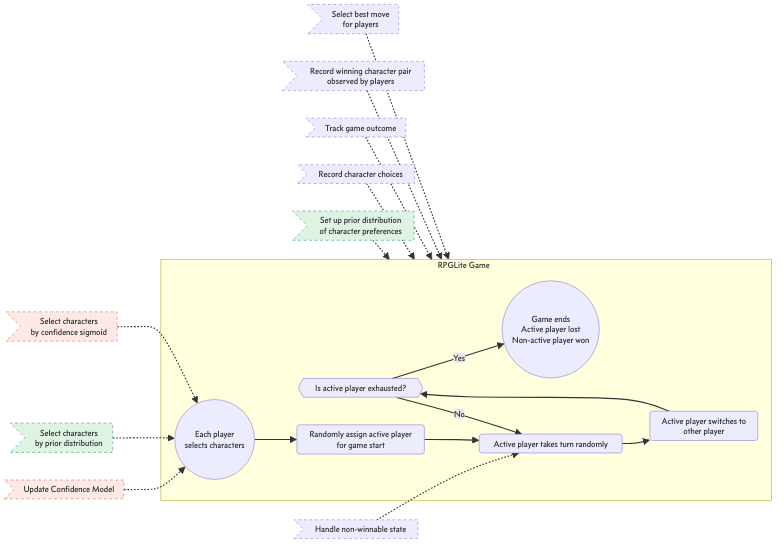
\includegraphics[width=\columnwidth]{60_optimisation_with_aspects/diagrams/aspect_applied_model.png}
  \caption{A flowchart describing a simulated game of RPGLite, and all aspects woven into the game to implement the various models of learning. Some aspects should not be woven together in the same experimental run, as they implement different models of learning.}
  \label{fig:all_aspects_applied}
\end{figure}


\subsection{Aspects for Model Improvement}\label{subsec:aspects_improving_model}

\subsubsection{Ensuring the Best Move is Played}\label{aspect_to_ensure_best_move}

% We make sure players always make the best moves, because it reduces the space of
% situations where randomness can skew our results. An analysis of how well this
% reflects real-world player interactions can be found in \inline{Cite William's
% thesis for realism of players making perfect moves.}


Experiments model players' character selection rather than move selection as
explained in \cref{learning_model_definition}; however, in the naive model
players randomly select moves. This is liable to place players in
unrealistically weak positions, as players are unlikely to make obviously poor
moves such as skipping a potentially useful turn. This is a concern when
modelling players learning to select characters because the learning model
relies on a causal relationship between what is observed (characters which most
reliably win games) and behavioural change (players choosing those characters).
If selecting random moves causes simulated players to lose games when they would
have won them when selecting moves realistically then move selection would
affect character selection. Realistic character selection and move selection are
therefore related.

Players of RPGLite usually selected moves optimally. In the majority of cases
\citet{kavanagh2021gameplay} found that players chose the best move available to
them: \emph{``\textelp{} the majority of actions taken were optimal, with a cost of
0.0. In total 73\% of the player's season 1 actions and 77.8\% of their season 2
actions were optimal.''}\footnote{Different seasons of RPGLite are discussed in
more depth in \cref{seasons_of_rpglite}.} Move selection can be realistically
modelled in around \(\frac{3}{4}\) of cases by selecting the best move at every
opportunity. This behaviour is implemented in an aspect by performing a lookup on
the dataset of action costs defined by \citet{kavanagh2021gameplay} and
selecting the known-optimal move in every case. This is woven into the naive
model's \lstinline{get_moves_from_table} function, which looks up moves from the
table of valid moves produced by \citet{kavanagh2021thesis}. It is invoked after
the function runs and alters its return value to include only the optimal move,
rather than all possible moves. Its source is included in
\cref{fig:best_move_aspect_source} as an example of the aspects implemented for this
thesis.\inline{Include a reference to the repo for the experiments' source code
so folk can see the other aspects too.}

\begin{figure}[h]
  \centering
  \lstinputlisting[style=footnotesize_python]{60_optimisation_with_aspects/snippets/select_best_move_aspect.py}
  \caption{An example of the implementation of an aspect for developing
  experiments around the naive model. This aspect ensures that the optimal move
  is selected by replacing the return value of \lstinline{get_moves_from_table}
  with the optimal move the function returned.}
  \label{fig:best_move_aspect_source}
\end{figure}

The aspect selecting optimal moves handles another concern of move
selection. As simulated players' behaviours are augmented to select universally
optimal moves, an anomaly in the dataset was identified. In some games, optimal
play results in infinite loops: players can arrive in a state where they would
skip turns mutually and indefinitely.

This occurs because barbarians deal more damage once they lose a sufficient
number of hit points. As a result, dealing damage to a barbarian can result in
their having an opportunity to win in one move rather than two in certain health
states. Both players can concurrently exist in this state. Therefore, both
players' optimal move is to skip their turn. \citeauthor{kavanagh2021gameplay}
note that such states were reached in 64 cases in real-world play but real-world
players never skipped their turn. To better mimic real-world play, the aspect
returns random moves if the previous two moves in a game skipped. Such a state
indicates that the game reached a state where neither player would deal damage
to the other when making optimal moves.


\subsubsection{Handle Game States with no Viable Moves}

A consequence of playing games using only optimal moves is that unexpected
states can occur: the dataset of possible moves produced by
\citet{kavanagh2021thesis} maps game states to moves a player may make, but not
all states exist in the dataset. This is because the dataset was produced
through model checking with the aim of identifying the cost of an action regards
its impact on a player's chance of winning. If a loss is guaranteed, all moves
have a 0\% chance of winning; the model checker which produced the dataset of
available moves therefore identified that the outcome of the game is already
determined in those cases, and produced no possible moves for them. 

The winning player in this situation is the player who made the previous move,
as the now-active player has no moves with a chance of winning above 0\%. This
logic is added to the model through an aspect which handles exceptions raised by
move selection, catching errors caused by an invalid table lookup. After
identifying that the exception indicates that the state does not exist (in this
case the relevant exception is Python's \lstinline{KeyError}), the aspect
handles the exception by assigning the losing player's characters 0 health and
swapping active players. The game proceeds with the losing player taking the
following turn. As this turn starts with the active (losing) player having 0
health, the game ends as expected.


\subsection{Aspects for Instrumentation}\label{subsec:aspects_instrumenting_model}

\subsubsection{Update Model of Confidence}
\label{confidence_model_aspect_impl_writeup}

As described in \cref{subsec:confidence_model}, confidence is modelled as a
Birch curve. This aspect updates a player's level of confidence using the birch
curve when a game ends. It is woven as a prelude to the naive model's
\lstinline{choose_character_pair} function, so that confidence is updated for
each player before it is used for character pair selection.

The aspect updates a value in the model's environment which represents the
confidence of the player selecting a character pair. The aspect uses the model's
environment to find parameters such as players' initial confidence or the value
of the curve's shape parameter $c$. The implementation of the aspect updating
the confidence model is given in
\cref{fig:update_confidence_model_aspect_source}. This implementation is edited
for readability, as the version used when running experiments contained
debugging code and additional logic used by other experiments which were
attempted but abandoned.

\begin{figure}[h]
  \centering
  \lstinputlisting[style=footnotesize_python]{60_optimisation_with_aspects/snippets/update_confidence_curve_aspect_edited.py}
  \caption{An example of the implementation of an aspect tracking model state.
  This aspect updates the value of a player's confidence model and is woven as
  prelude to the naive model's \lstinline{choose_character_pair} function.}
  \label{fig:update_confidence_model_aspect_source}
\end{figure}

\subsubsection{Record Prior Distribution of Character Preferences}
\label{record_prior_distribution}

To implement the prior distribution model, the character pair preferences of the
player being simulated must be calculated. The prelude aspect implementing this
is shown in \cref{fig:prelude_before_learning_by_prior_distribution}. Computing
this distribution involves loading, parsing, and filtering the entire dataset of
RPGLite gameplay data. However, the program running experiments must load this
dataset to construct the parameters controlling the simulation --- in particular
\lstinline{training_data} and \lstinline{testing_data}, introduced later in
\cref{model_parameters} --- so to avoid duplicating this work, the values are
retrieved from the stack frames of the function which constructed the model
parameters. The players being simulated and games played by them are identified
by their variable names in the stack frame, and their distribution is calculated
through a convenience function,
\lstinline{find_distribution_of_charpairs_from_players_collective_games}, the
implementation of which is given in
\cref{fig:calculating_charpair_distribution}.

\begin{figure}[hp]
  \centering
  \begin{lstlisting}[style=footnotesize_python]
def prelude_before_learning_by_prior_distribution(target, actor, gamedoc, env, *args, **kwargs):
  # Before we fuzz, we need to make sure the prior distribution is set up in the game's environment.
  # Calculate and inject it if it's not already there.
  if 'simulation prior distribution' not in env:
      # Grab players and games from an earlier stack frame
      # (avoids weaving an aspect to collect the info)
      frame_to_find_name = "generate_charpair_distributions"
      for frameinfo in inspect.stack():
          if frameinfo.function == frame_to_find_name:
              break
      games = frameinfo.frame.f_locals['games']
      players = frameinfo.frame.f_locals['players']

      from experiment_base import find_distribution_of_charpairs_from_players_collective_games
      env['simulation prior distribution'] = find_distribution_of_charpairs_from_players_collective_games(players, games)
  \end{lstlisting}
  \caption{The prelude aspect calculating the distribution of character pairs selected by the real-world player being simulated, which is reproduced by simulated players using the prior distribution model.}
  \label{fig:prelude_before_learning_by_prior_distribution}
\end{figure}

\begin{figure}[hp]
  \begin{lstlisting}[style=footnotesize_python]
def find_distribution_of_charpairs_from_players_collective_games(players, gameset):
    distribution = dict()
    for player in players:
        player_distribution = find_distribution_of_charpairs_for_user_from_gameset(player, gameset)
        for charpair, count in player_distribution.items():
            distribution[charpair] = distribution.get(charpair, 0) + count

    return distribution

def find_distribution_of_charpairs_for_user_from_gameset(player, gameset):
    charpair_distribution = dict()
    for game in gameset:
        # Game is from RPGLite's real-world mongodb if it has a `_id` field.
        if '_id' in game:
            game = convert_gamedoc_to_tom_compatible(game)

        if player in game:
            char1 = game[player]['chars'][0][0]
            char2 = game[player]['chars'][1][0]
            pair = char1 + char2 if char_ordering[char1] < char_ordering[char2] else char2 + char1
            charpair_distribution[pair] = charpair_distribution.get(pair, 0) + 1

    return charpair_distribution
    
def convert_gamedoc_to_tom_compatible(gamedoc):
    '''
    We use this to convert a game document from MongoDB to the kind generated by the simulation, for ease of comparison.
    '''
    new_gamedoc = deepcopy(gamedoc)

    new_gamedoc['players'] = gamedoc['usernames']
    new_gamedoc[gamedoc['usernames'][0]] = dict()
    new_gamedoc[gamedoc['usernames'][1]] = dict()
    new_gamedoc[gamedoc['usernames'][0]]['chars'] = [gamedoc['p1c1'], gamedoc['p1c2']]
    new_gamedoc[gamedoc['usernames'][1]]['chars'] = [gamedoc['p2c1'], gamedoc['p2c2']]

    return new_gamedoc
  \end{lstlisting}
  \caption{The implementation of a helper function which calculates the distribution of character pairs from the games a player completed.}
  \label{fig:calculating_charpair_distribution}
\end{figure}

This allows the calculation of the distribution to be separated from the change
to players' character pair selection. Separating these into two different
aspects allows them to use different join points: this aspect is a prelude and
operates before character pairs are chosen, whereas the change made to character
selection is performed using a ``within''-style fuzzer from \pdsf{}. The
\lstinline{if} statement at the beginning of the aspect, as shown in
\cref{fig:prelude_before_learning_by_prior_distribution}, avoids calculating the
distribution more than once.
\revnote{
  Bit thin maybe? I'm not sure what to say about the prior distribution model.
  It's so simple! Hopefully this is sufficient.
}



\subsubsection{Record Character Pair Choices}
It is important to keep track of the characters chosen by simulated players, as
this data is required to analyse the outcome of the experiments outlined in
\cref{experiments_introduced_briefly}. However, the naive model makes no special
accommodation for the collection of character choices made by players. Character
choices could be calculated by iterating through the list of completed games
after a simulation is complete, filtering for games relating to a specific
player. However, the collection of character selection data can be simplified by
tracking what was played at the end of a game. This is achieved with with an
aspect which observes the character pairs played in a completed game, and
appends each players' chosen pairs to their own list. This aspect is applied
after its join point executes (an ``encore'' in PyDySoFu
parlance, as discussed in \cref{subsec:prior_work_theatre}).

There are many ways to collect this data, aspectually or otherwise; however, the
simplicity of collecting information mid-process without requiring modification
of a base model demonstrates the flexibility of an aspectual augmentation of
models and simulations as an approach. Collection of chosen character pairs
mid-simulation is an opportune example of this convenience.

\subsubsection{Track Detailed Outcomes of Games}
\label{subsubsec:detailed_game_outcome_tracking_aspect}

Similarly to the recording of character pair choices, the outcomes of games must
be tracked. This information is important as an input the learning model, as
successes and failures observed by players for each character pair constitute
what they learn as ``good'' and ``bad'' character pair selections. 

As with character pair choices, the naive model was not engineered with the
intention of providing this information specifically. However, the model is
easily instrumented to collect such information at many suitable points. As with
recording a player's chosen character pairs, an ``encore'' aspect was
implemented which records wins and losses observed for character pairs on game
end. Specifically, the aspect models players observing character pairs which won
at the end of a game, lost at the end of a game, and also pairs which were
uninvolved in the game. This requires a list of outcomes (wins, losses, and
neither) for every player, for every character pair. The lists of observed
outcomes for a given character pair record \lstinline{True} for a winning pair,
\lstinline{False} for a losing pair, and \lstinline{None} for a character which
was not involved in the game's outcome. Each player observes the relevant state
for every character at the end of any game they play. Provisions were made in
the implementation of this aspect for a player only paying attention to their
own outcomes (i.e. only recording whether their own pair won or lost, without
consideration for their opponent's outcome), though in practice all simulations
were performed with players observing both their own outcomes and those of their
opponents.

\subsubsection{Record Winning Pair observed by Players on Game End}
\label{subsubsec:aspect_to_observe_winning_pair}

The simple model of learning makes use of a distribution of winning teams to
simulate learning (the implementation of which is explained in
\cref{subsubsec:learning_by_picking_from_distribution_of_wins_with_confidence}).
Rather than coalescing the more complex dataset collected as described in
\cref{subsubsec:detailed_game_outcome_tracking_aspect} to achieve the desired
format, another aspect can be applied to collect the data in a simpler format
directly.

An aspect was implemented which models players observing winning character
pairs on game end and collects the data in a simple list of character pairs
which won games, rather than a mapping of character pairs to game end
states as described in \cref{subsubsec:detailed_game_outcome_tracking_aspect}.
Character pairs which lose games or are not involved are not recorded for the
purpose of the alternative model of learning.
\revnote{This aspect needs a bit more of an explanation. Maybe a code snippet?}

% TODO: Section / subsection for models of learning
\subsection{Aspects Implementing Models of Learning}\label{subsec:aspects_modelling_learning}


The aspects described at this point mostly correct move selection, handle
exceptions which can arise from this, and instrument the model for experimental
observation. What remains is to describe the implementation of aspects which
encode behavioural changes: the prior distribution model, which selects
character pairs by drawing from a distribution of character pair choices known
before the simulation runs, and the learning model, which selects character
pairs using a character's observations of which pairs typically win or lose
games. \revnote{Clumsy, rework if there's time.}


\subsubsection{Character Selection using Prior Distribution}
\label{prior_distribution_aspect_description}

The prior distribution model alters character selection by changing the
distribution of character pairs selected from when simulating RPGLite play. The
distribution they choose from is changed to reflect the distribution selected by
the player being simulated. Another aspect, explained earlier in
\cref{record_prior_distribution}, calculates that distribution and stores it in
the simulation's environment. The role of this aspect is to use that
distribution when selecting character pairs at the beginning of a game.

\begin{figure}
  \centering
  \begin{lstlisting}[style=footnotesize_python]
def fuzz_learning_by_prior_distribution(steps, target, actor, env, *args, **kwargs):
    get_choices_from_prior_dist_injected_code = '''
players = _context['players']
games = _env['games']

distribution = _env['simulation prior distribution']
possible_choices = list()
for pair, count in distribution.items():
    for _ in range(count):
        possible_choices.append(pair)

char_class_map = {
    "K": Knight,
    "A": Archer,
    "R": Rogue,
    "W": Wizard,
    "H": Healer,
    "B": Barbarian,
    "M": Monk,
    "G": Gunner
}
chars_chosen = [char_class_map[char] for char in choice(possible_choices)]
'''
    to_inject = ast.parse(get_choices_from_prior_dist_injected_code)
    return [steps[0]] + to_inject.body + [steps[2]]
  \end{lstlisting}
  \caption{The implementation of the prior distribution model's change to player
  behaviour, implemented as a \pdsf{} fuzzer which inserts character pair
  selection logic into the \lstinline{choose_chars} function of the naive model
  to select character pairs using the distribution taken from RPGLite gameplay
  data in an earlier aspect.}
  \label{fig:prior_distribution_implementation}
\end{figure}


The aspect implementing the prior distribution's behaviour change is shown in
\cref{fig:prior_distribution_implementation}. It is implemented using \pdsf{}'s
fuzzers (or ``within''-style aspects) to insert additional logic within
character pair selection rather than prepending or appending logic to it. Logic
is added by modifying the target program's abstract syntax tree (\emph{``AST''}),
a native representation of Python code. The steps of the fuzzer's target ---
provided by \pdsf{} as the fuzzer's first argument --- are nodes of the AST
representing the function definition of the target. The target in this case is
\lstinline{choose_chars}. An implementation of this function is given in
\cref{fig:choose_chars_implementation_annotated_with_steps}, edited to show how
the lines in the function definition map to values in the \lstinline{steps}
argument of the fuzzer.

\begin{figure}
  \begin{lstlisting}[style=footnotesize_python]
def choose_chars(_actor, _context, _env):
    if _actor not in _context: # First "step", or steps[0]
        _context[_actor] = dict()

    chars_chosen = sample(characters, 2) # Second "step", or steps[1]
    _context[_actor]['chars'] = [c() for c in chars_chosen] # Third "step", or steps[2]
  \end{lstlisting}
  \caption{The naive model's \lstinline{choose_chars} function, which selects
  character pairs for a player to play a game with randomly.}
  \label{fig:choose_chars_implementation_annotated_with_steps}
\end{figure}

Python code to select character pairs using the desired distribution is written
in a multi-line string and parsed into an AST. This code:

\begin{itemize}
\item Takes the distribution of character pairs from the game's environment,
represented as a map of two-letter strings (for example, ``KA'', representing
the pair \lstinline{Knight}, \lstinline{Archer}) to the number of times a player
selected the pair represented by that string,
\item Constructs a list, \lstinline{possible_choices}, which contains the
two-character string identifying a character pair as many times as the character
pair was chosen by a player,
\item Creates a map of letters to classes implementing the characters those
letters represent (for example, ``K'' maps to the \lstinline{Knight} class),
\item Sets the \lstinline{chars_chosen} variable to a list of two classes, by
selecting a character pair from the \lstinline{possible_choices} list at random
and adding the class implementing each character in that pair to the
\lstinline{chars_chosen} list.
\end{itemize}

This leaves \lstinline{chars_chosen} in the same state as it would have been
without the application of the prior distribution model: a list of two
character-implementing classes. However, those classes were selected using the
distribution produced from RPGLite gameplay data. The AST nodes produced by
parsing this code are used to replace the second step in
\lstinline{choose_chars}. The rest of the function logic remains the same. The
changed AST nodes are returned by the fuzzer and compiled by \pdsf{}, ensuring
that the modified function definition is executed and so changing player
behaviour.



\subsubsection{Character Selection using confidence sigmoid}
\label{subsubsec:learning_by_picking_from_distribution_of_wins_with_confidence}

The first model of learning applied through aspect orientation draws on
character pairs a simulated player observed to have won games (as recorded by
the relevant instrumenting aspect, discussed in
\cref{subsubsec:aspect_to_observe_winning_pair}). The record of previously
winning character pairs defines a probability mass function by selecting a
character with equal probability to their rate of appearance in the history of
winning characters.

Selecting a character based on this distribution is gated by a confidence model
as described in \cref{subsec:confidence_model}. If a simulated player's
confidence model indicates insufficient experience to found decisions on,
players will instead select characters randomly, effectively exploring their
space of possible choices. By doing so, players have the time and opportunity to
observe many matchups between different character pairs. Time to observe
matchups is important because some character pairs may only present a strong
choice if played against specific alternatives. We can imagine a character pair
which is extremely effective against 50\% of pairs, but extremely likely to lose
games played against the remaining 50\% of possible opponents. Without exploring
possible matchups, a player may lack observations which would inform them about
whether a character pair is effective in general, or in a narrow set of
circumstances. A confidence model encouraging early exploration promotes the
experience of a wide variety of matchups, avoiding this issue.

Another concern early exploration mitigates is that simulated players need
opportunities to build well-rounded priors: if a character pair is never
selected by any player, experienced players basing their character pair choices
on those which previously win games cannot include pairs which were never
selected, because they will never have had the opportunity to win games at all.

This aspect was implemented as an ``around'' aspect in PyDySoFu's parlance,
allowing it to apply additional logic before and after its join point. It could
equally appropriately have been implemented as an ``encore'', applying logic
only after its join point had executed; the aspect discards the random selection
made by the base model unless the simulated player lacks confidence. Either
implementation can return a different character pair choice to the join point's
caller, allowing the chosen character pair to effectively be overridden, and so
allowing the aspect-applied RPGLite model to proceed executing as it would
otherwise; the only difference being the pair of characters ``chosen'' by the
simulated player whose behaviour was augmented.





\section{Model Implementation Details}
\label{sec:optimisation_with_aspects_experimental_design}

The aspects described in \cref{aspects_applied_section} are used to investigate
whether \aop{} can be used to augment models, add new behaviours and parameters
to them, and successfully do so across different models. The results of these
investigations are presented in \cref{chap:experimental_results}; some details
about the implementation of those experiments are given first in this section.

The parameters used to control experiments are introduced in
\cref{model_parameters}. The representation of experiments' results is given in
\cref{representing_results_of_an_experimental_run}. The statistical methods used
to evaluate those results are explained in \cref{measuring_charpair_similarity}.
Finally, the methods used to control simulated players' interactions with their
environments to produce reliable datasets are explained in
\cref{subsec:controlling_state_space_exploration}.



\subsection{Model Parameters}
\label{model_parameters}

Many parameters are used to control simulated play of RPGLite. They affect the
impact of the learning model and the scaffolding which runs simulations, for
example by determining the number of simulated players. Parameters which control
an experimental run are collected in the \lstinline{ModelParameters} class,
shown in \cref{fig:model_parameters_class}. Defining these values in a class
helps to identify them in the codebase, and defines all variables which are used
when optimising the model.

\begin{figure}[tp]
    \centering
    \lstinputlisting[style=footnotesize_python]{60_optimisation_with_aspects/snippets/ModelParameters.py}
    \caption{A class defining the parameters of the model of learning RPGLite which vary when optimising for a given player. For layout \& space reasons, some methods of minor significance are removed.}
    \label{fig:model_parameters_class}
\end{figure}

As there are a significant number of parameters and many have a straightforward
impact on simulated play, a complete description is given in
\cref{appendix_model_parameters} in the interest of readability. A description
is given here for parameters which have a non-obvious effect, or are the focus
of the experimental methodology in \cref{methodology_explained}, or are central
to the results given in \cref{sec:rq3} and \cref{sec:rq4}. Variables used in
these ways are:

\Needspace{3\baselineskip}
\begin{description}[style=multiline,leftmargin=4cm]
  \item[starting confidence] The initial value of the model's confidence curve.
  \item[assumed confidence plateau] A corresponding high value for the model's
  confidence curve. As the curve's growth rate is calculated to align with the
  number of games completed by the real-world player being simulated, and the
  curve asymptotically approaches 1, a high value is required which represents
  the expected confidence of a real-world player having played a significant
  number of games.
  \item[curve inflection relative to numgames] The proportion of games played by
  the real-world player being simulated at which the player's confidence
  curve should reach the parameter \\\lstinline{assumed_confidence_plateau}. This
  allows for control over the growth rate of the curve while linking the rate of
  growth to the number of games played by the real-world player being simulated;
  \item[C] The curve parameter of the confidence model's underlying birch curve;
  \item[prob bored] The probability that a player with confidence above
  \lstinline{assumed_confidence_plateau} becomes ``bored'' and stops playing
  RPGLite. These players are removed from the simulated playerbase and replaced
  with new players. This mechanism is discussed in further detail in
  \cref{subsec:controlling_state_space_exploration}.
  \item[advice] A list of tuples defining advice to weave when generating data.
  Pieces of advice are uniquely defined by a tuple containing the type of aspect
  to weave (such as \lstinline{"prelude"} or \lstinline{"error_handler"}), a
  string-represented regular expression defining the join point of the advice,
  and a \lstinline{callable} to use as an aspect when weaving the advice. As
  \lstinline{ModelParameters} instances are serialised to disk to persist
  experiment results and Python functions are not seralisable, this may also be
  a string value; strings are IDs of aspects, and are replaced with their
  corresponding aspect on deserialisation.
  \item[training data] The set of real-world games used as a training fold when
  optimising parameters for simulating a player. This is used when annealing
  toward optimal parameters for the learning model, and so is explained in more
  detail in \cref{methodology_explained}.
  \item[testing data] The set of real-world games used as a testing fold when
  optimising parameters for simulating a player. This is used when annealing
  toward optimal parameters for the learning model, and so is explained in more
  detail in \cref{methodology_explained}.
\end{description}



As these determine all variables affecting data generation, individual
experimental runs\footnote{Throughout this chapter, ``experimental run'' is used
to refer to the process of producing a simulated dataset for comparison against
training or testing folds taken from the dataset of completed RPGLite games.
Many experimental runs with different parameters are used to optimise a model.}
can therefore be reproduced using the class. The convenience method
\lstinline{run_experiment()}, shown in
\cref{fig:ModelParameters_run_experiment_method}, is provided to simplify
reproducing experimental runs with \lstinline{ModelParameters} objects. These
parameters are varied in some experimental runs to optimise the model and
represent individual players' learning to find a combination of parameters which
best represent a given player. The strategy for this optimisation is described
in \cref{methodology_explained}.

\begin{figure}[bp]
  \begin{center}
    \begin{lstlisting}[style=footnotesize_python]
class ModelParameters:

    # <snipped additional attributes and methods for space>

    def run_experiment(self, testing, correlation_metric):
        real, synthetic = generate_charpair_distributions(\
            rgr_control=self.rgr(testing=False),
            iterations=self.iterations(testing=False),
            games=self.training_data,
            players=self.players,
            birch_c=self.c,
            sigmoid_initial_confidence=self.starting_confidence,
            boredom_confidence=self.assumed_confidence_plateau,
            num_synthetic_players=self.number_simulated_players,
            boredom_period=self.boredom_period,
            prob_bored=self.prob_bored,
            advice=self.advice,
            *self.args,
            **self.kwargs)
        return Result(self, real, synthetic, correlation_metric, testing)
    \end{lstlisting}
  \end{center}
  \caption{The \lstinline{run_experiment()} method on the
  \lstinline{ModelParameters} class, which can be used to reproduce an
  experimental run from its parameters.}
  \label{fig:ModelParameters_run_experiment_method}
\end{figure}


\subsection{Representing the Result of an Experimental Run}
\label{representing_results_of_an_experimental_run}

As referenced in \cref{fig:ModelParameters_run_experiment_method}, a
\lstinline{Result} class is defined to collect the results of an experimental
run and simplify analysis of the distribution of character pair selection
produced. The implementation of the \lstinline{Result} class is given in
\cref{fig:Result_class}. This class is used in the analysis of the success of an
experimental run when selecting ideal experimental parameters for the simulation
of a real-world player.

A \lstinline{Result} is not the result of an entire experiment, or the ideal
parameters to simulate a given player. Instead, it represents the result of
attempting to generate realistic data for a player, which is defined by a
\lstinline{ModelParameters} attribute. Several \lstinline{Result} objects can be
compared against correlation statistics and probabilities of circumstantial correlation
(the \lstinline{statistic} and \lstinline{pval} properties respectively) using
the \lstinline{within_acceptable_bounds} method to
select an optimal set of parameters to simulate an RPGLite player. A technique
which uses these properties to determine optimal parameters is described in
\cref{methodology_explained}.


\begin{figure}[tp]
  \begin{center}
    \begin{lstlisting}[style=footnotesize_python]
from dataclasses import dataclass
@dataclass
class Result:
    params:ModelParameters
    real_distribution:list[float]
    simulated_distribution:list[float]
    correlation_metric:Optional[callable]
    testing: bool

    @property
    def pval(self) -> float:
        return self.correlation_metric(self.real_distribution, self.simulated_distribution).pvalue

    @property
    def statistic(self) -> float:
        return self.correlation_metric(self.real_distribution, self.simulated_distribution).statistic

    def within_acceptable_bounds(self, pval_threshold:float, statistic_threshold:float) -> bool:
        return self.pval < pval_threshold and self.statistic > statistic_threshold
    \end{lstlisting}
  \end{center}
  \caption{The \lstinline{Result} class used to collect results of experimental
  runs and evaluate their success.}
  \label{fig:Result_class}
\end{figure}


\subsection{Quantifying Similarity of Character Pair Selection}
\label{measuring_charpair_similarity}

To measure the results of experiments in \cref{chap:experimental_results}, many
datasets are generated (with differing model parameters in the case of the
learning model) and are compared against a player's completed games to determine
which generated dataset is most similar to the empirical one. The distribution
of the naive model should exhibit no bias as character pairs are chosen
randomly; simulated play with advice woven is expected to exhibit more
``realistic'' character pair preferences than the naive model as a result of the
advice applied. The similarity between a player's character pair preferences and
those of simulated players are determined using a rank correlation measurement.

Many rank correlation measurements exist. A non-paremetric measurement is
required for measuring the correlation of character pair distributions.
Non-parameteric correlation measurements make no assumptions about the
distribution of data; the alternative is to use a parametric measurement, which
would be selected based on the distribution in the data being compared. The
distribution of character pair preferences is unknown, so to avoid assuming a
distribution which is universally applicable to all players' interaction with
RPGLite a non-parametric correlation measurement is chosen.

Two common non-parametric rank-correlation measurements are
\citeauthor{spearman_rho_measurement_of_association}'s
\rho{}~\cite{spearman_rho_measurement_of_association} and
\citeauthor{kendall_tau_rank_correlation}'s
\tau{}~\cite{kendall_tau_rank_correlation}. The differences between these
methods can affect measurements of character pair preference.
\citeauthor{spearman_rho_measurement_of_association}'s \rho{} accounts for the
magnitude of difference between ranks, and is calculated as $\rho = 1 - \frac{6
\sum (d^{2}_{i})}{n(n^{2}-1)}$, where $d_{i}$ is the difference in the rank
of the $i^{th}$ observation in each dataset and $n$ is the total number of
datapoints in a dataset. \citeauthor{kendall_tau_rank_correlation}'s \tau{}
accounts only for their ordering. It can be calculated as $\tau = \frac{C - D}{C
+ D}$, where $C$ is the count of pairs with the same rank
(\emph{``concordant''}), and $D$ the count of pairs with differing ranks
(\emph{``discordant''}).

To choose an appropriate measure for comparing character pair distributions,
they can be related to potential patterns in those distributions. As a player is
likely not to select many character pairs once they have developed preferences
(if at all), a slight increase in selecting uncommon character pairs within a
simulation could incur a significant increase in the rank of those pairs. This
would have a more significant impact on \rho{} than on \tau{}, as the larger
difference in rank is squared in the calculation. Character pairs' rankings may
also have small differences between the two distributions but similar positions
relative to each other. For example, most character pairs could have ranks only
1 position apart between the distributions. This would have an outsized impact
on \tau{}, as relative positioning affects concordance, but the square of a
small difference in rank remains relatively small, meaning that \rho{} would be
less affected by this pattern. A choice of correlation metric is thus a choice
of what correlation means: it can reflect preference of character pairs relative
to each other, or ``forgive'' small relative preference deviations and impose a
greater cost on the scale of disagreement on a given rank instead.

%% === I began making the below to illustrate the examples in the above chapter
%      but couldn't figure out how to format it properly. Keeping the stubs
%      incase I revisit.

% \begin{figure}
%   \centering
%   \begin{minipage}{0.45\textwidth}
%   \begin{tabular}{l r r}
%     \emph{Character Pair} & \emph{Games Played} & \emph{Rank}    \\
%     KA & 25 & 1 \\ 
%     KW & 15 & 2 \\
%     AW &  5 & 3 \\
%     BK &  3 & 4 \\
%     BA &  2 & 5 \\
%     BW &  1 & 6 \\
%   \end{tabular}
%   \end{minipage}
%   \begin{minipage}{0.45\textwidth}
%   \begin{tabular}{l r r}
% \end{figure}

To prioritise the preservation of the order of a ranking character pair
preferences are compared using \tau{}. Unfavoured character pairs' ranks might
be affected greatly by a small difference in the number of games played, because
unfavoured character pairs play few games. A small difference in selection count
is therefore more likely affect the rank of those pairs. Minimising rank
difference is sensitive to RPGLite's random nature for this reason. Preserving
the ordering of character pair selection is also important when considering
favoured pairs, as most games are likely to be played with a small number of
favoured pairs. Much as large differences in unfavoured pairs' ranks can be
caused by random chance, small differences in the ranks of favoured pairs are
indicative of a player's preferences. An appropriate correlation measurement
must take this into account. Small differences in the ranks of favoured pairs
would have a less signifiant impact on \rho{} than on \tau{}: \rho{} accounts
for the square of the difference in rank, which remains small for small
differences. Experimental results are calculated using \tau{} in
\cref{chap:experimental_results} for this reason: \tau{} prioritises accurately
simulating a player's preferences when selecting character pairs, which is the
aim of the experiments, and so is the more appropriate measurement.


\subsection{Controlling State Space Exploration}
\label{subsec:controlling_state_space_exploration}

The model of confidence grows monotonically as described in
\cref{subsec:defining_our_models_of_learning}, which affects simulated players'
exploration of possible character pairs. The learning model uses confidence as a
probability that character pairs are selected based on experience. As character
pairs which are not played cannot win games, pairs which are not selected for
play cannot be chosen by the learning model as it relies on a player's
historical observations, which could lead to inaccurate simulation if the
unchosen pair is the player's preference. To counter this possibility, two
mechanisms are introduced to control state space exploration: ``initial
exploration'' and ``boredom''.

Initial exploration is a threshold number of games a simulated player must
complete before the confidence model determines whether aspects should change
player behaviour. The earning model's impact on player behaviour is gated on
both a player's level of confidence and the number of games played. This allows
players to enough games that later decisions directed by the learning model can
make ``informed'' decisions, having explored the possible options. The length of
the initial exploration phase for any player is given as an integer number of
games by the \lstinline{initial_exploration} parameter when generating data.

Boredom is a mechanism which solves a problem introduced by some combinations of
model parameters: if the confidence model's growth rate and curve parameter are
high, player confidence raises sharply, with the effect that simulated players
are unlikely to explore the state space. A situation can arise where the
simulation's metagame falls into a local optimum where the entire playerbase
collectively observe many historical wins for some character pairs because of a
disproportionately high rate of random selection when players explore the space
of possible character pairs. This can be overcome by introducing new players
into the playerbase over time. New players are guaranteed to explore the state
space due to the initial exploration phase. The randomly selected character
pairs played in this time mean that veteran players will play games with
character pairs which otherwise could not have been selected. This reinforces
existing preferences when novel character pairs are weaker than veteran players'
preferences, and weakens existing preferences if veteran players are exposed to
novel character pairs which are likely to win games played against their
preferred pairs. By disrupting the simulation's metagame boredom mitigates
potential issues with random play while allowing simulated players to learn over
time.

Players are eligible to be removed from the playerbase when their model of
confidence reaches a threshold defined by the
\lstinline{assumed_confidence_plateau} parameter. Each player is removed with
probability \lstinline{prob_bored} once this threshold is reached, allowing some
confident players to remain in the playerbase for a long time. Any player who is
removed is immediately replaced with a new one, so the playerbase has a constant
size. The \lstinline{boredom_period} parameter determines the number of games
between these checks, and the mechanism can be disabled entirely using the
\lstinline{boredom_enabled} parameter.




% \section{Discussion}
% \label{sec:optimisation_with_aspects_discussion}

% A closing discussion on what we found, and how the research question was
% answered.

% Also, note the weaknesses of the approach.

% \begin{itemize}
%   \item More games could have lead to a more accurate result
%   \item It'd be interesting to use the models to ``learn'' other things too,
%     such as move selection / mistakes made
%   \item Would like to reproduce across multiple different systems, not just
%     RPGLite. Maybe developers like we did in the CAISE paper, maybe aspects that
%     aren't learning like degraded modes. Could be interesting to model a complex
%     adaptive system with aspects representing rule changes. Could be interesting
%     to demonstrate other uses of aspectually augmented systems, like introducing
%     new rules to a cellular automaton.
% \end{itemize}
